%This work is licensed under the Creative Commons Attribution-NonCommercial-NoDerivs 3.0 United States License. To view a copy of this license, visit http://creativecommons.org/licenses/by-nc-nd/3.0/us/ or send a letter to Creative Commons, 444 Castro Street, Suite 900, Mountain View, California, 94041, USA.

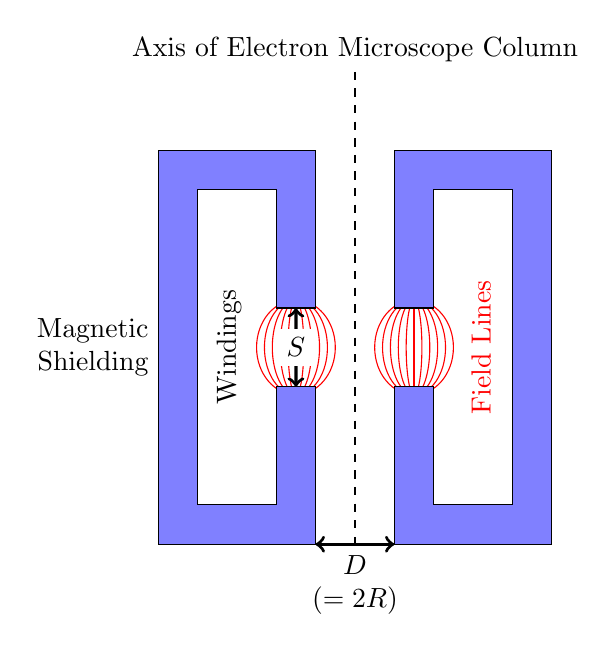
\begin{tikzpicture}
  \foreach \n in {0,0.1,...,0.6}{
    \draw [red] (0.75,-0.5) ellipse [x radius=\n,y radius=0.6];
  }
  \foreach \n in {0,0.1,...,0.6}{
    \draw [red] (-0.75,-0.5) ellipse [x radius=\n,y radius=0.6];
  }
  \draw [fill=blue!50] 
    (-0.5,0)
    -- ++(0,2)
    -- ++(-2,0)
    -- ++(0,-5)
      node [pos=0.5,left,align=right] {Magnetic\\Shielding}
    -- ++(2,0)
    -- ++(0,2)
      coordinate [pos=0] (D left)
    -- ++(-0.5,0)
      coordinate [pos=0.5] (S top)
    -- ++(0,-1.5)
    -- ++(-1,0)
    -- ++(0,4)
    -- ++(1,0)
    -- ++(0,-1.5)
    -- ++(0.5,0)
      coordinate [pos=0.5] (S bottom)
    -- cycle
  ;
  \draw [fill=blue!50] 
    (0.5,0)
    -- ++(0,2)
    -- ++(2,0)
    -- ++(0,-5)
    -- ++(-2,0)
    -- ++(0,2)
      coordinate [pos=0] (D right)
    -- ++(0.5,0)
    -- ++(0,-1.5)
    -- ++(1,0)
    -- ++(0,4)
    -- ++(-1,0)
    -- ++(0,-1.5)
    -- cycle
  ;
  \draw [thick, dashed]
    (0,3)
    -- (0,-3)
      node [pos=0,above] {Axis of Electron Microscope Column}
  ;
  \draw [very thick,<->] 
    (S top) 
    -- (S bottom)
      node [pos=0.5,fill=white] {$S$}
  ;
  \draw [very thick,<->] 
    (D left) 
    -- (D right)
      node [below,pos=0.5,align=center] {$D$\\$(=2R)$}
  ;
  \node [rotate=90] at (-1.6,-0.5) {Windings};
  \node [red,rotate=90] at (1.6,-0.5) {Field Lines};
\end{tikzpicture}
